\chapter{M\'odulo de Odontograma (Registro Dental)}

\section{Descripci\'on General}

El m\'odulo de odontograma permite el registro y seguimiento de la
condici\'on dental de los pacientes. Utiliza el \textbf{sistema de
numeraci\'on Triadan} modificado para identificar cada diente, con
soporte para perros (42 dientes) y gatos (30 dientes).

\section{Sistema de Numeraci\'on Triadan}

El sistema Triadan asigna un n\'umero de 3 d\'{\i}gitos a cada diente:

\begin{itemize}[leftmargin=*]
    \item \textbf{Primer d\'{\i}gito:} Cuadrante (1 y 2 = maxilar superior,
          3 y 4 = mand\'{\i}bula inferior; 1 y 3 = lado derecho, 2 y 4 =
          lado izquierdo).
    \item \textbf{Dos \'ultimos d\'{\i}gitos:} Posici\'on del diente
          (incisivos 01-03, canino 04, premolares 05-08, molares 09-11).
\end{itemize}

\begin{lstlisting}[style=typescript, caption=Numeracion Triadan desde constantes compartidas]
export const TOOTH_NAMES: Record<number, string> = {
  101: 'I1', 102: 'I2', 103: 'I3', 104: 'C',
  105: 'P1', 106: 'P2', 107: 'P3', 108: 'P4',
  109: 'M1', 110: 'M2',
  // ... demas dientes
};

export const DOG_TEETH = [101, 102, 103, 104, 105, 106, 107, 108,
  109, 110, 201, 202, 203, 204, 205, 206, 207, 208, 209, 210,
  301, 302, 303, 304, 305, 306, 307, 308, 309, 310, 311,
  401, 402, 403, 404, 405, 406, 407, 408, 409, 410, 411];
// 42 dientes para perros

export const CAT_TEETH = [101, 102, 103, 104, 106, 107, 108, 109,
  201, 202, 203, 204, 206, 207, 208, 209,
  301, 302, 303, 304, 305, 306, 307,
  401, 402, 403, 404, 405, 406, 407];
// 30 dientes para gatos
\end{lstlisting}

\section{Estados Dentales}

Cada diente puede tener uno de 12 estados:

\begin{longtable}{|l|l|l|}
\hline
\textbf{Estado} & \textbf{Etiqueta} & \textbf{Color} \\
\hline
healthy & Sano & verde \\
fractured & Fracturado & rojo \\
missing & Ausente & gris \\
worn & Desgastado & naranja \\
calculus & C\'alculo/Sarro & amarillo \\
gingivitis & Gingivitis & rosa \\
mobility & Movilidad & p\'urpura \\
retained\_deciduous & Retenido & azul \\
root\_remnant & Resto radicular & gris oscuro \\
caries & Caries & marr\'on \\
pulp\_exposure & Exposici\'on pulpar & rojo oscuro \\
other & Otro & negro \\
\hline
\end{longtable}

\section{Server Actions}

\subsection{Upsert Pattern}

\begin{lstlisting}[style=typescript, caption=upsertDentalRecord - Inserta o actualiza segun exista]
export async function upsertDentalRecord(
  patientId: number,
  data: { teeth: ToothCondition[]; notes?: string },
) {
  const clinicId = await getCurrentClinicId();

  // Verifica si ya existe un registro dental para este paciente
  const existing = await db
    .select({ id: schema.dentalRecords.id })
    .from(schema.dentalRecords)
    .where(eq(schema.dentalRecords.patientId, patientId))
    .limit(1);

  if (existing[0]) {
    // UPDATE
    await db
      .update(schema.dentalRecords)
      .set({
        teeth: data.teeth,
        notes: data.notes ? { general: data.notes } : undefined,
        updatedAt: new Date(),
      })
      .where(eq(schema.dentalRecords.id, existing[0].id));
  } else {
    // INSERT
    await db.insert(schema.dentalRecords).values({
      clinicId,
      patientId,
      teeth: data.teeth,
      notes: data.notes ? { general: data.notes } : {},
    });
  }

  revalidatePath(`/patients/${patientId}`);
  revalidatePath(`/odontogram/${patientId}`);
}
\end{lstlisting}

\subsection{Otras Funciones}

\begin{itemize}[leftmargin=*]
    \item \texttt{getDentalRecords(patientId)} --- Lista todos los registros.
    \item \texttt{getLatestDentalRecord(patientId)} --- \'Ultimo registro
          (usando \texttt{ORDER BY createdAt DESC LIMIT 1}).
    \item \texttt{getDentalToothSummary(patientId)} --- Solo el array de
          dientes del \'ultimo registro.
\end{itemize}

\section{Almacenamiento}

Los datos dentales se almacenan como JSONB:

\begin{lstlisting}[style=typescript, caption=Tipos ToothCondition y formato JSONB]
export interface ToothCondition {
  toothNumber: number;   // 101-411 (Triadan)
  status: ToothStatus;   // healthy, fractured, etc.
  notes?: string;        // Notas opcionales por diente
}

// Ejemplo de datos almacenados:
[
  { "toothNumber": 104, "status": "fractured",
    "notes": "Fractura completa con exposicion pulpar" },
  { "toothNumber": 105, "status": "calculus",
    "notes": "Sarro moderado" }
]
\end{lstlisting}

\begin{figure}[H]
    \centering
    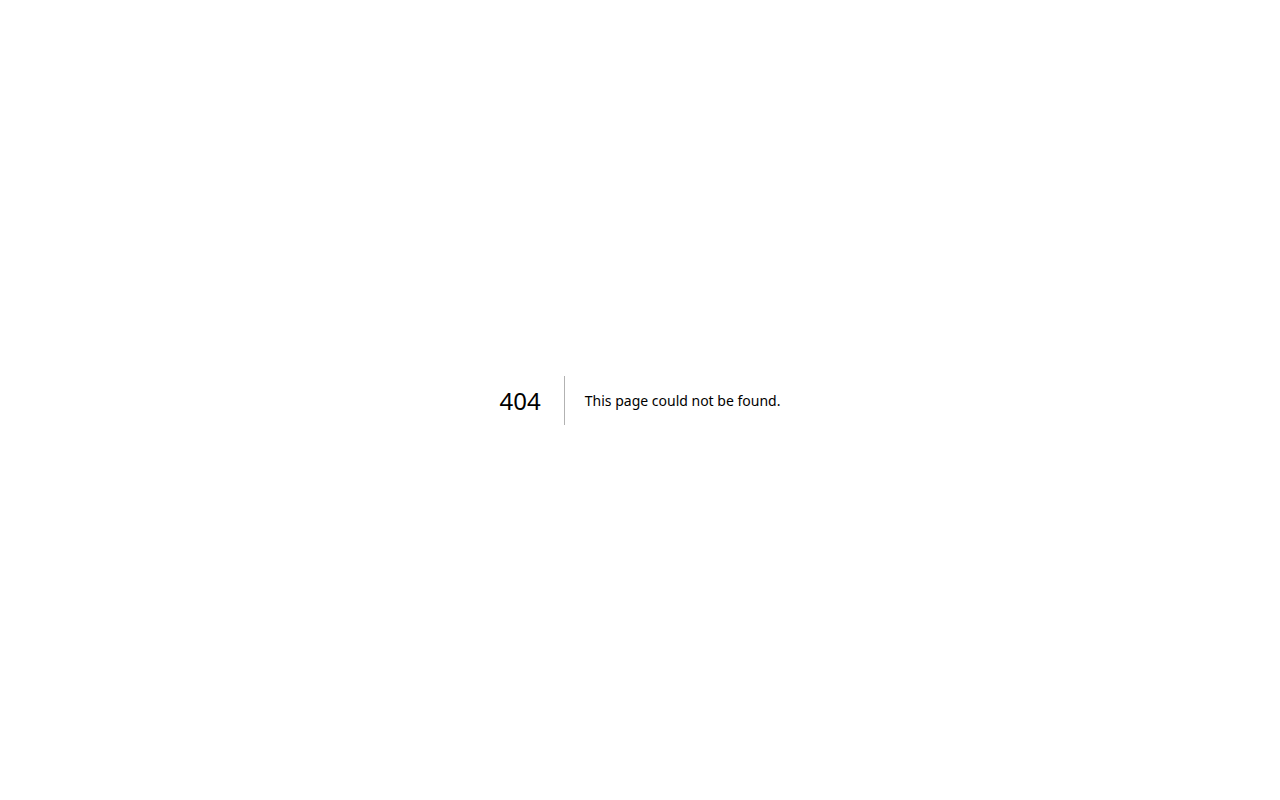
\includegraphics[width=\textwidth]{img/vet-odontogram.png}
    \caption{Registro dental con sistema de numeracion Triadan}
    \label{fig:odontograma}
\end{figure}
